\section{Systematic uncertainties}
\label{systematics}
Several systematic uncertainties are applied to the simulated signal efficiency to account for uncertainty in the signal yields arising from possible mismodeling of the detector conditions and response. The following subsections describe each systematic uncertainties in turn, and Table~\ref{systematics_summary} summarizes all systematic uncertainties applied to the simulated signal.

\begin{table}
\noindent \centering{}\topcaption{\label{systematics_summary}Systematic uncertainties in the signal efficiency for all years and channels. The mean is provided in cases where the uncertainty varies by signal sample. Uncertainties in the same row are treated as correlated among the years of data taking, except for the displaced tracking and muon pixel hit efficiencies, where the 2016 uncertainty is treated as uncorrelated with the 2017 and 2018 uncertainties.}
\begin{tabular}{lrrr}
\hline
Systematic uncertainty & 2016 & 2017 & 2018\tabularnewline
\hline
\textit{Integrated luminosity}      & 1.8\% & 1.8\% & 1.8\%  \tabularnewline
\textit{Pileup} \\ 
 - $\Pe\Pgm$ channel    & 0.5\%   & 0.6\%  & 0.5\%  \tabularnewline
 - $\Pe\Pe$ channel     & 0.5\%   & 0.9\%      & 0.8\%  \tabularnewline
 - $\Pgm\Pgm$ channel   & 0.2\%   & 0.1\%     & 0.2\%  \tabularnewline
\textit{Displaced tracking efficiency}  & 14\%  & 5.8\%   & 2.4\% \tabularnewline
\textit{Trigger efficiency} \\
- $\Pe\Pgm$ channel, electrons   & 1.6\%  & 1.3\%   & 1.2\%   \tabularnewline
- $\Pe\Pgm$ channel, muons       & 1.6\%  & 1.4\%   & 1.2\%   \tabularnewline
- $\Pe\Pe$ channel               & 10\%   & 13\%    & 19\%  \tabularnewline
- $\Pgm\Pgm$ channel             & 1.2\%  & 1.0\%   & 1.1\%   \tabularnewline
\textit{Muon trigger efficiency at large \ad} \\
- $\Pe\Pgm$ channel, muons       & 20\%  & 20\%   & 20\%   \tabularnewline
- $\Pgm\Pgm$ channel             & 20\%  & 20\%   & 20\%   \tabularnewline
\textit{Lepton identification and isolation} \\
- $\Pe\Pgm$ channel, electrons   & 1.2\%     & 3.6\%   & 3.5\%  \tabularnewline
- $\Pe\Pgm$ channel, muons       & 0.05\%  & 0.07\%  & 0.06\% \tabularnewline
- $\Pe\Pe$ channel               & 2.4\%     & 7.2\%    & 7.0\%  \tabularnewline
- $\Pgm\Pgm$ channel             & 0.10\%  & 0.14\%  & 0.12\% \tabularnewline
\textit{Muon pixel hit efficiency} \\
- $\Pe\Pgm$ channel, muons       & 32\%  & 12\%  & 16\% \tabularnewline
- $\Pgm\Pgm$ channel             & 73\%  & 23\%  & 30\% \tabularnewline
\textit{Lepton \ad correction} \\
- $\Pe\Pgm$ channel, electrons     & \NA   & 0.001\%   & 0.001\%  \tabularnewline
- $\Pe\Pgm$ channel, muons         & \NA   & 0.003\%  & 0.001\% \tabularnewline
- $\Pe\Pe$ channel                 & \NA   & 0.11\%   & 0.11\% \tabularnewline
- $\Pgm\Pgm$ channel               & \NA   & 0.11\%   & 0.11\% \tabularnewline
\hline
\end{tabular}
\end{table}

\subsection{Integrated luminosity}
The integrated luminosities of the 2016, 2017, and 2018 data-taking periods are individually known with uncertainties in the 2.3--\SI{2.5}{\percent} range~\cite{CMS:lumi2016,CMS:lumi2017,CMS:lumi2018}, while the total Run~2 (2016--2018) integrated luminosity has an uncertainty of \SI{1.8}{\percent}, the improvement in precision reflecting the uncorrelated time evolution of some systematic effects.

\subsection{Pileup}
The simulation of pileup events assumes a total inelastic proton-proton cross section of \SI{69.2}{\milli\barn} with an associated uncertainty of \SI{5}{\percent}~\cite{Sirunyan:2018nqx}. The systematic uncertainty arising as a result of the modeling of pileup events is estimated by varying the cross section of the minimum bias events by \SI{5}{\percent} when generating the target pileup distributions. The pileup weights are recomputed with these new distributions and applied to the simulated events to obtain the variation in the yields in the inclusive signal region. The average uncertainty is between 1 and \SI{2}{\percent}. We treat these uncertainties as \SI{100}{\percent} correlated across the three years of data taking.

\subsection{Displaced tracking efficiency}
The systematic uncertainty associated with the modeling of the displaced tracking efficiency is derived from a dedicated study using cosmic-ray muons. Following the results of the study presented in Appendix~\ref{displaced_tracking_eff}, we assign \SI{14.1}{\percent}, \SI{5.8}{\percent}, and \SI{2.4}{\percent} systematic uncertainties in 2016, 2017, and 2018, respectively. Because the CMS pixel detector was upgraded between 2016 and 2017 data taking, we treat the 2017 and 2018 systematic uncertainties as fully correlated and the 2016 systematic uncertainty as uncorrelated with 2017 and 2018.

\subsection{Trigger efficiency}
The trigger efficiency systematic uncertainty is given by the uncertainty in the measured trigger efficiency scale factors (see Section~\ref{trig_eff}). These uncertainties are \SI{1}{\percent} or less for the \Pe\Pgm\ and $\Pgm\Pgm$ channels and about \SI{10}{\percent} for the \Pe\Pe\ channel. In addition, we have studied the trigger efficiency in signal as a function of \ad for events in the trigger \pt plateau. To cover the change observed in the muon trigger efficiency over the full \ad range, we assign an additional \SI{20}{\percent} uncertainty.

We treat the trigger efficiency uncertainties as \SI{100}{\percent} correlated across the three years of data taking.

\subsection{Lepton ID and isolation}
To find the systematic uncertainty associated with the corrections to the lepton ID and isolation, we fluctuate the lepton scale factors up and down by their uncertainty and observe the change in the event yields in the inclusive signal region. The average uncertainty for electrons is about \SI{3}{\percent} in the \Pe\Pgm\ channel and about \SI{7}{\percent} in the \Pe\Pe\ channel, while the average uncertainty for muons is $< \SI{1}{\percent}$. We treat these uncertainties as \SI{100}{\percent} correlated across the three years of data taking.

\subsection{Muon pixel hit efficiency}
The requirement in the muon ID that muons have at least one pixel hit could in principle have some appreciable \ad dependence, so we perform a dedicated study to ensure that we account for any differences in \ad dependence between data and simulation. Figure~\ref{muon_pixel_hit_eff} shows the efficiency of this requirement in cosmic simulation and \texttt{NoBPTX} data (described in appendix~\ref{displaced_tracking_eff}) as a function of muon \ad. For events in the denominator of these plots, we require  that at least 2 global, PF muons have $\abs{\eta}<1.0$, $\pt>\SI{25}{\GeV}$, no displaced vertices in the tracker material, $\abs{d_z}<\SI{15}{\cm}$, and pass all the tight ID criteria except the pixel hit requirement. We also require the muons to be separated by $\DR>0.2$. The events in the numerator must pass the same requirements in addition to the requirement that the muons have at least one pixel hit. From this plot, we calculate the mean efficiency to identify the muons in the simulated signal events using the same procedure as is used for the displaced tracking efficiency systematic uncertainty described in Appendix~\ref{displaced_tracking_eff}. We repeat the procedure in both cosmic simulation and in \texttt{NoBPTX} data, and using the ratio of these two efficiencies, we derive the relative systematic uncertainty in the signal. The average uncertainty is about \SI{16}{\percent} (\SI{32}{\percent}) in the \Pe\Pgm\ (\Pgm\Pgm) channel. As the pixel detector was upgraded after 2016, the 2017 and 2018 systematic uncertainties are treated as fully correlated while the 2016 uncertainty is treated as uncorrelated with the 2017 and 2018 uncertainties.

\begin{figure}
\centering
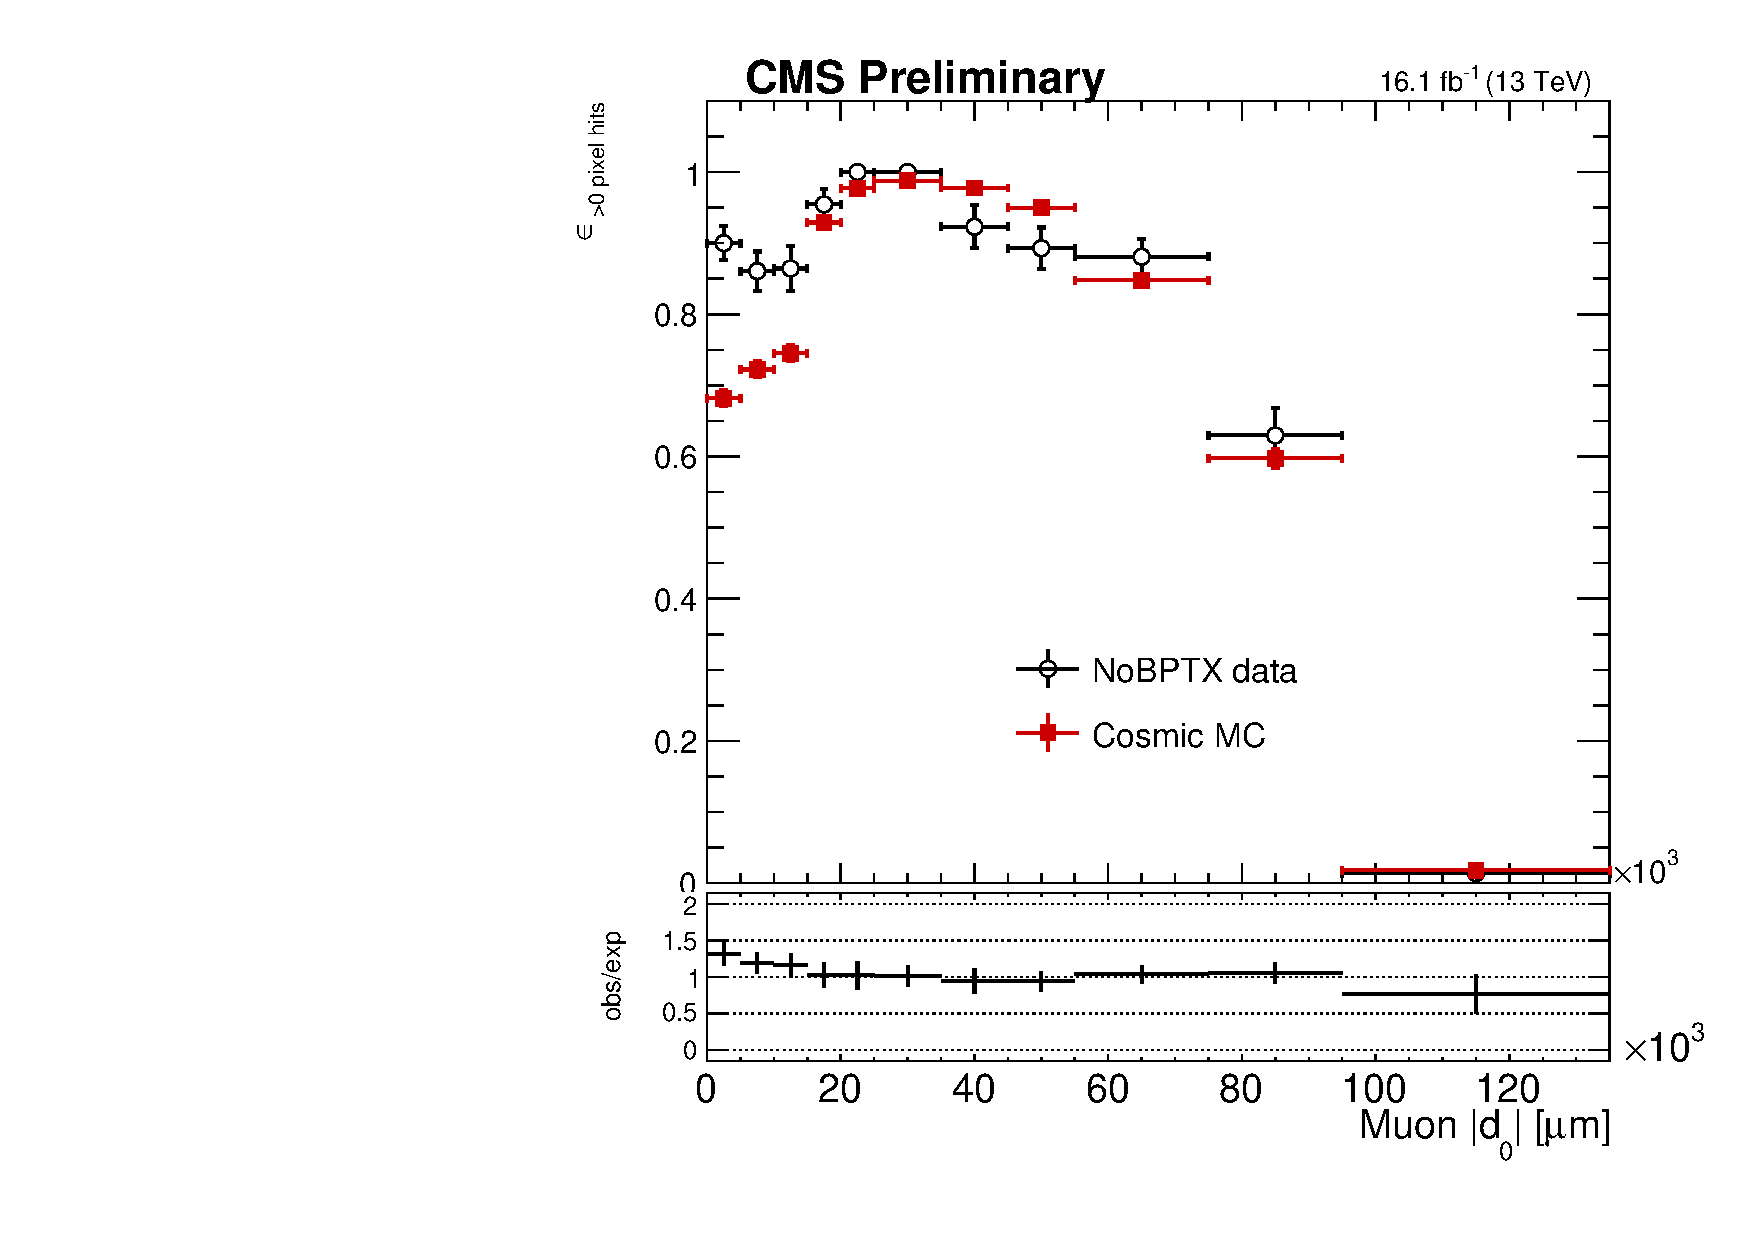
\includegraphics[width=0.32\textwidth]{figures/systematics/muon_pixel_hit_eff/muonAbsD0_100000um_variableBins_coarse_2016.pdf}
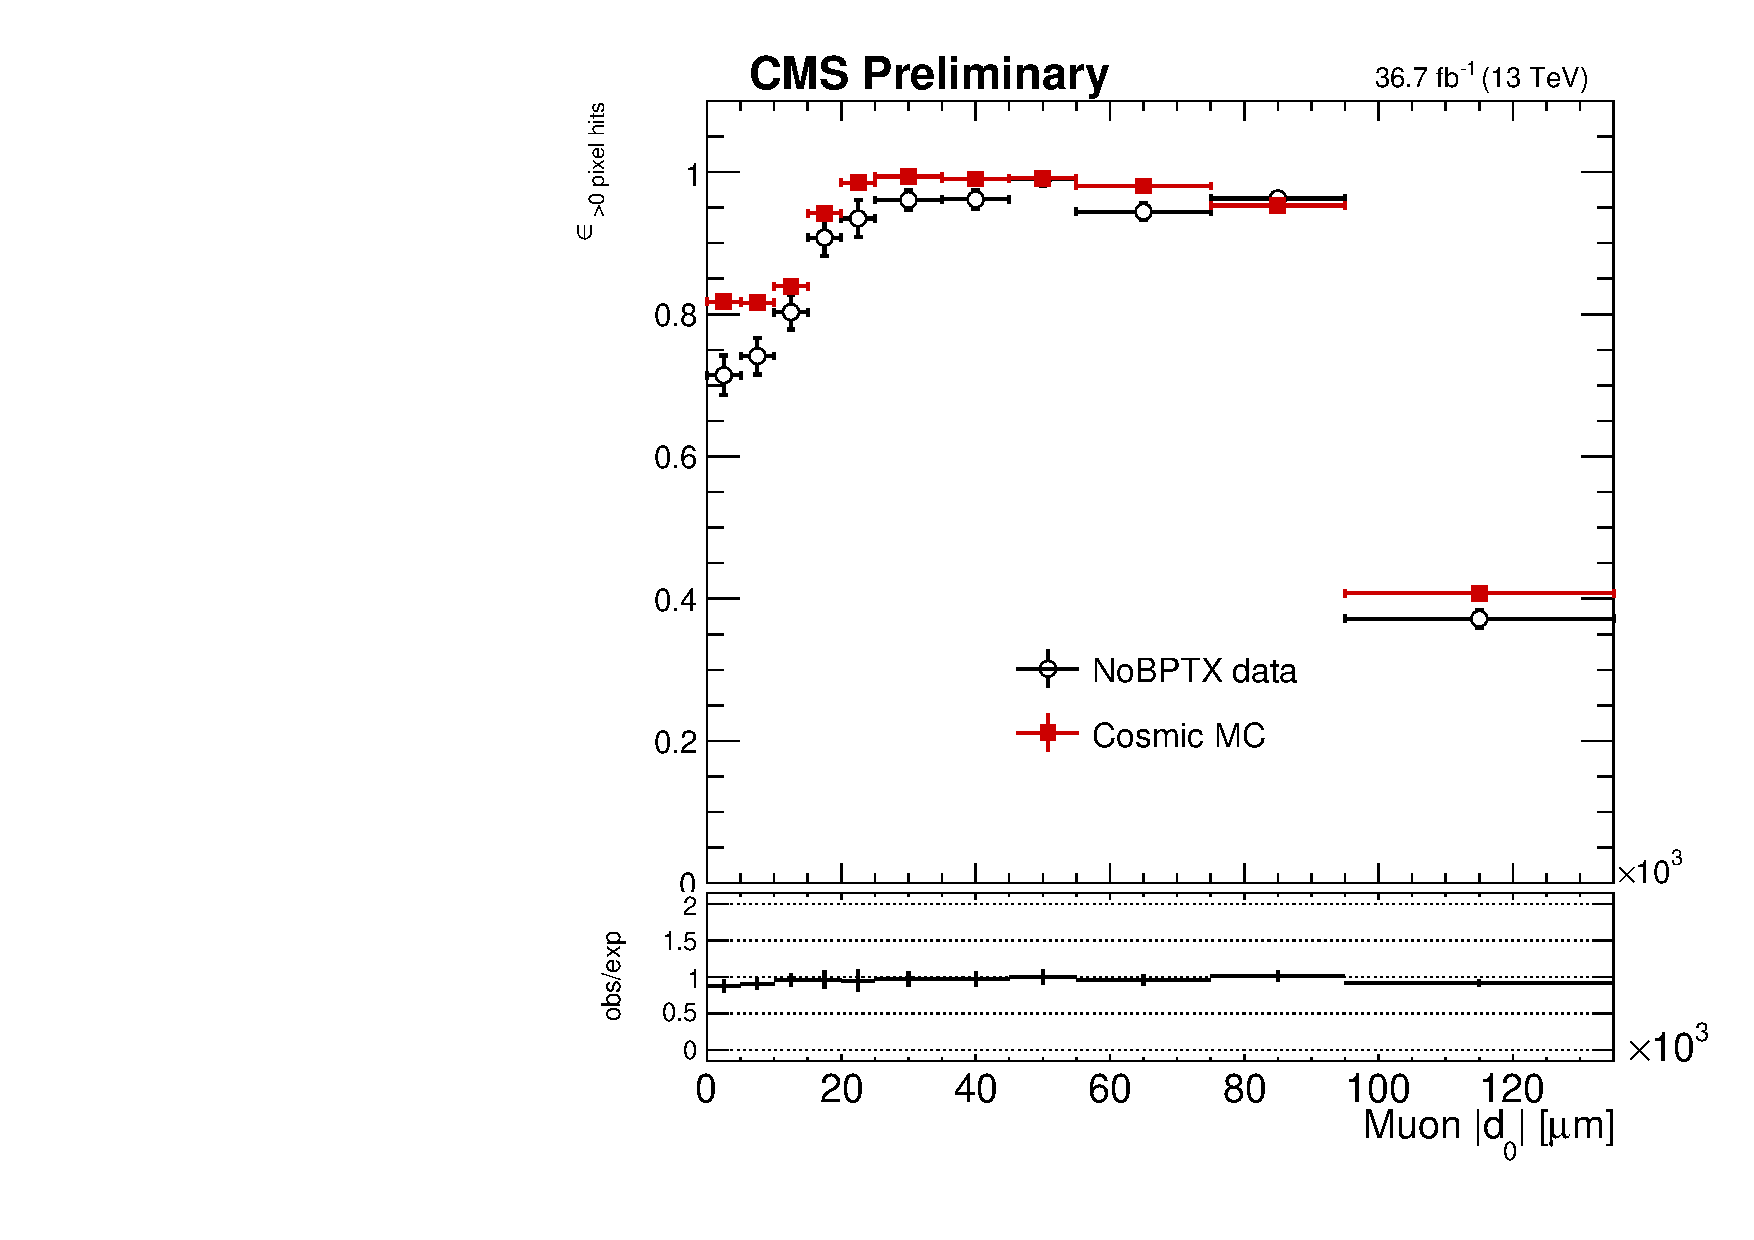
\includegraphics[width=0.32\textwidth]{figures/systematics/muon_pixel_hit_eff/muonAbsD0_100000um_variableBins_coarse_2017.pdf}
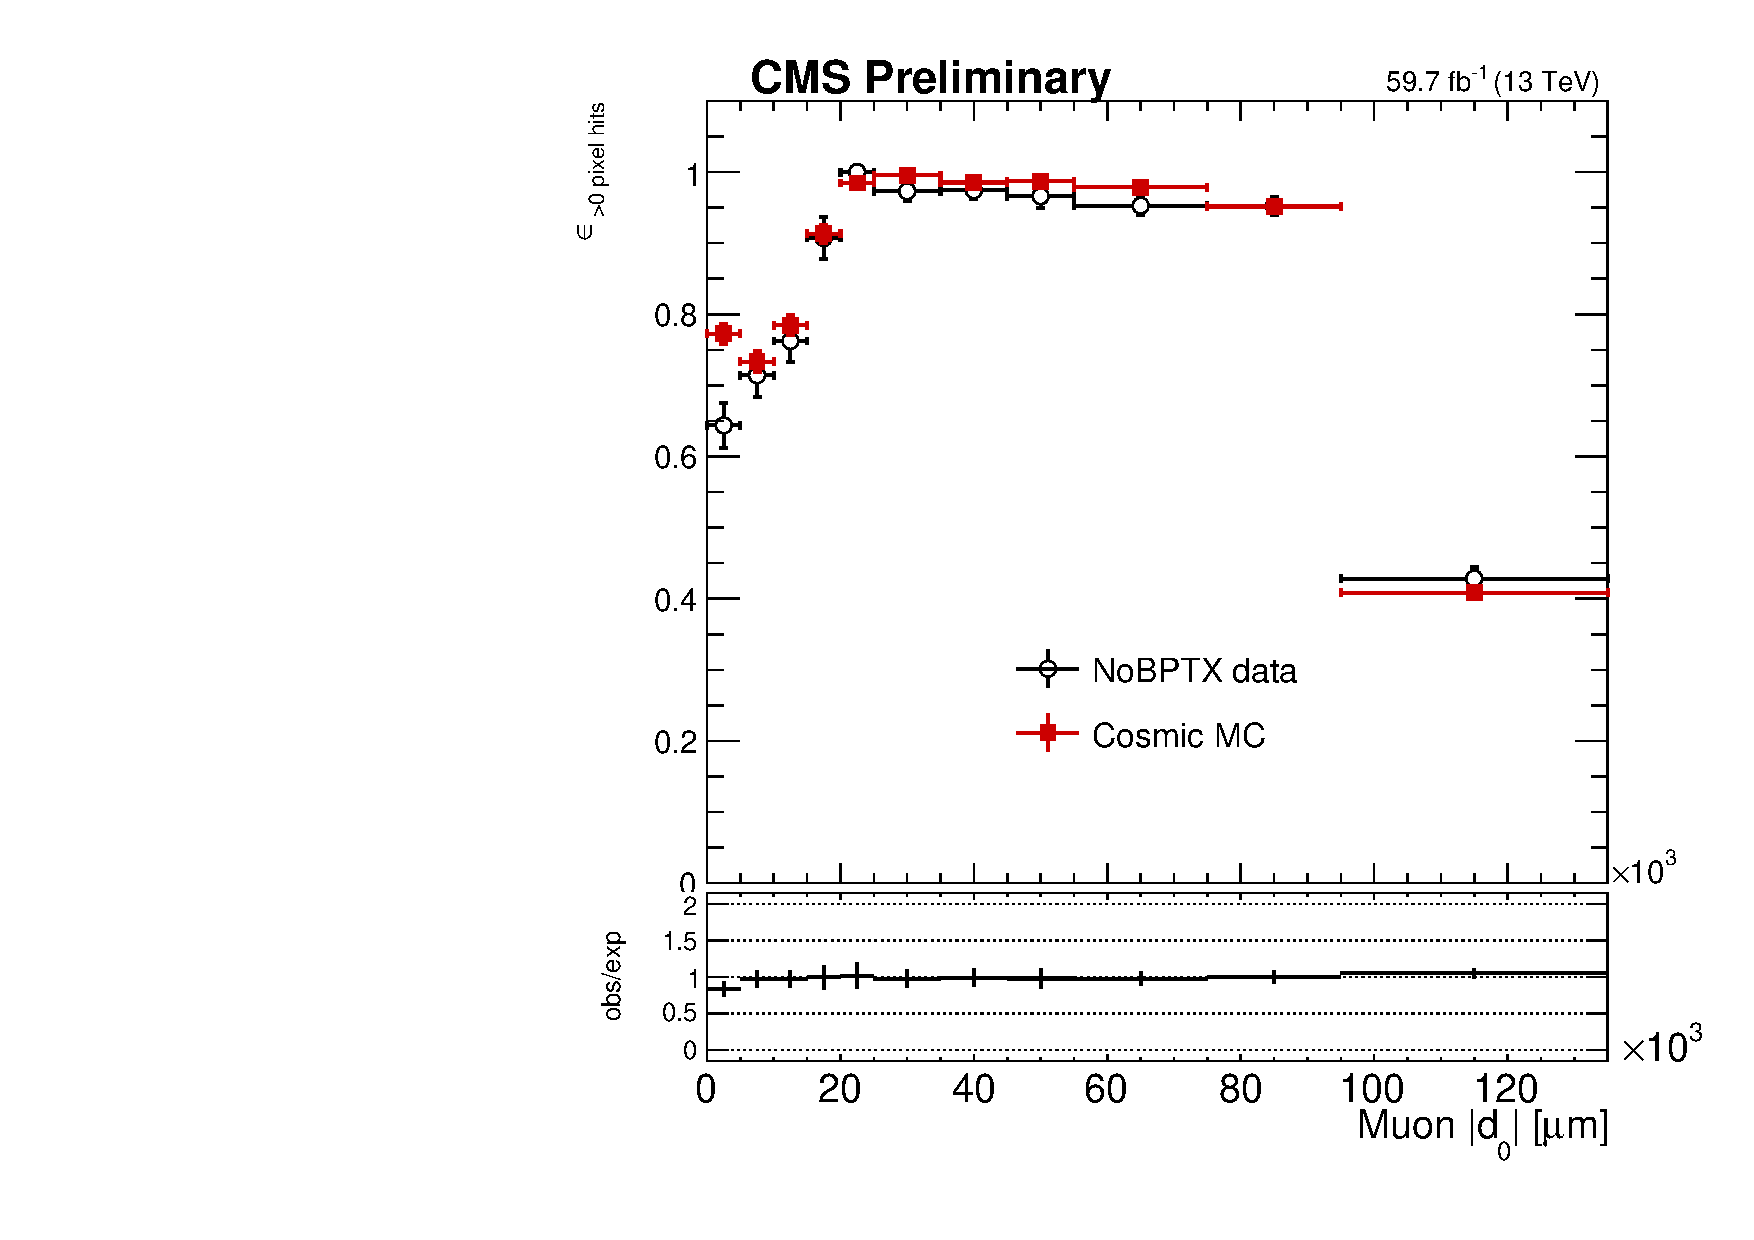
\includegraphics[width=0.32\textwidth]{figures/systematics/muon_pixel_hit_eff/muonAbsD0_100000um_variableBins_coarse_2018.pdf}
\caption{The pixel hit efficiency as a function of muon \ad in simulated cosmic ray events and \texttt{NoBPTX} data in 2016 (left), 2017 (center), and 2018 (right) conditions.}
\label{muon_pixel_hit_eff}
\end{figure}

\subsection{Lepton $d_0$ resolution}
To find the systematic uncertainty associated with the corrections to the lepton $d_0$ (see Section~\ref{d0_smearing}), we fluctuate the lepton $d_0$ corrections up and down by their uncertainty and observe the change in the event yields in the inclusive signal region. The average uncertainty is $<\SI{1}{\percent}$. We treat these uncertainties as \SI{100}{\percent} correlated in 2017 and 2018. No $d_0$ correction or systematic uncertainty is needed for 2016 simulation.

\pagebreak